Proces podejmowania decyzji, polegający na wybieraniu najlepszej opcji z 
zestawu możliwych, jest obecny w niemal każdym możliwym zadaniu człowieka. Z
tego powodu, badania nad podejmowaniem decyzji są konieczne i ważne nie tylko w 
teorii decyzji, ale również w takich dziedzinach jak zarządzanie, badania
operacyjne,  polityka, psychologia społeczna, sztuczna inteligencja, soft 
computing i tak dalej. Oczywistym jest, że porównywanie różnych działań w 
zależności od ich zalet, w wielu przypadkach, jest niemożliwe do osiągnięcia 
przy pomocy jednego kryterium lub jednej osoby. Dlatego też, proces decyzyjny 
rozpatrywany jest jako grupowe podejmowanie decyzji.

Niezaprzeczalnym faktem jest, że problemy stawiane grupie w większości pochodzą 
z życia wziętych sytuacji. W tych problemach jest do dyspozycji zbiór alternatyw
rozwiązujących problem oraz grupa ekspertów, cechująca się doświadczeniem i 
wiedzą, która stara się osiągnąć wspólne rozwiązanie. Aby rozwiązać problem, 
eksperci muszą przejść przez dwa etapy: proces osiągania konsensusu oraz proces 
selekcji.

W poniższym rozdziale te dwa etapy zostaną dokładnie opisane. Przedstawiony
będzie model iteracyjny, który wykorzystuje proces osiągania konsensusu i proces
selekcji. Na końcu wprowadzone zostaną elementy dynamiki, które mogą pojawić się
w procesie podejmowania decyzji oraz propozycje poradzenia sobie z tym.

\section{Model iteracyjny}
W grupowym podejmowaniu decyzji można wyróżnić dwa procesy prowadzące do
uzyskania ostatecznego rozwiązania: proces osiągania konsensusu oraz proces
selekcji. Pierwszy zajmuje się osiągnięciem maksymalnie najwyższego porozumienia
pomiędzy ekspertami. Zwykle proces ten prowadzony jest przez tak zwanego
moderatora i jest  wykonywany przed procesem selekcji. Proces porozumienia jest
bardzo ważnym krokiem, ponieważ wspomaga uzyskanie rozwiązań o wysokim stopniu
konsensusu wśród  ekspertów, co zazwyczaj jest pożądaną własnością. Drugi proces
odnosi się do sposobu uzyskania zbioru alternatyw jako rozwiązań z opinii oraz
ocen każdej z alternatyw przedstawionych przez ekspertów.

\subsection{Definicja problemu}
Przed przystąpieniem do poszczególnych kroków trzeba formalnie zdefiniować 
problem. Z punktu widzenia modelu, nie jest to opis czy postawione pytanie. 
Typowy wieloosobowy, wielokryteriowy problem składa się z następujących 
elementów:

\begin{description}
  \item[Zbiór alternatyw $ \mathcal{X} = \{ x_1, \dotsc, x_n \}.$] Zbiór
  $\mathcal{X}$ odpowiada skończonej i dyskretnej liście więcej niż jednej
  możliwości. Odpowiednie właściwości (lub atrybuty) każdej alternatywy mogą być
  ilościowe lub jakościowe.
  
  \item[Zbiór kryteriów $ \mathcal{C} = \{ c_1, \dotsc, c_n \}.$] Zbiór
  $\mathcal{C}$ zawiera dwa lub więcej kryteriów. Każdemu kryterium odpowiada
  punkt widzenia, zgodnie z którym alternatywy są oceniane i porównywane. Mogą
  one mieć charakter ilościowy lub jakościowy i posiadać większą lub mniejszą
  wagę dla decyzji.
  
  \item[Zbiór decydentów $ \mathcal{E} = \{ e_1, \dotsc, e_n \}.$] Zbiór
  $\mathcal{E}$ zawiera więcej niż jednego eksperta. Zazwyczaj każdy z ekspertów
  ma własną perspektywę, motywację i priorytety, które mogą prowadzić do
  sprzecznych opinii i preferencji. Ponadto każdy decydent odgrywa rolę w
  procesie decyzyjnym, która jest określana przez stopień wiedzy, doświadczenia
  oraz intuicji w danej sprawie.

\end{description}

\subsection{Proces porozumienia (konsensusu)}

\begin{figure}[ht]
  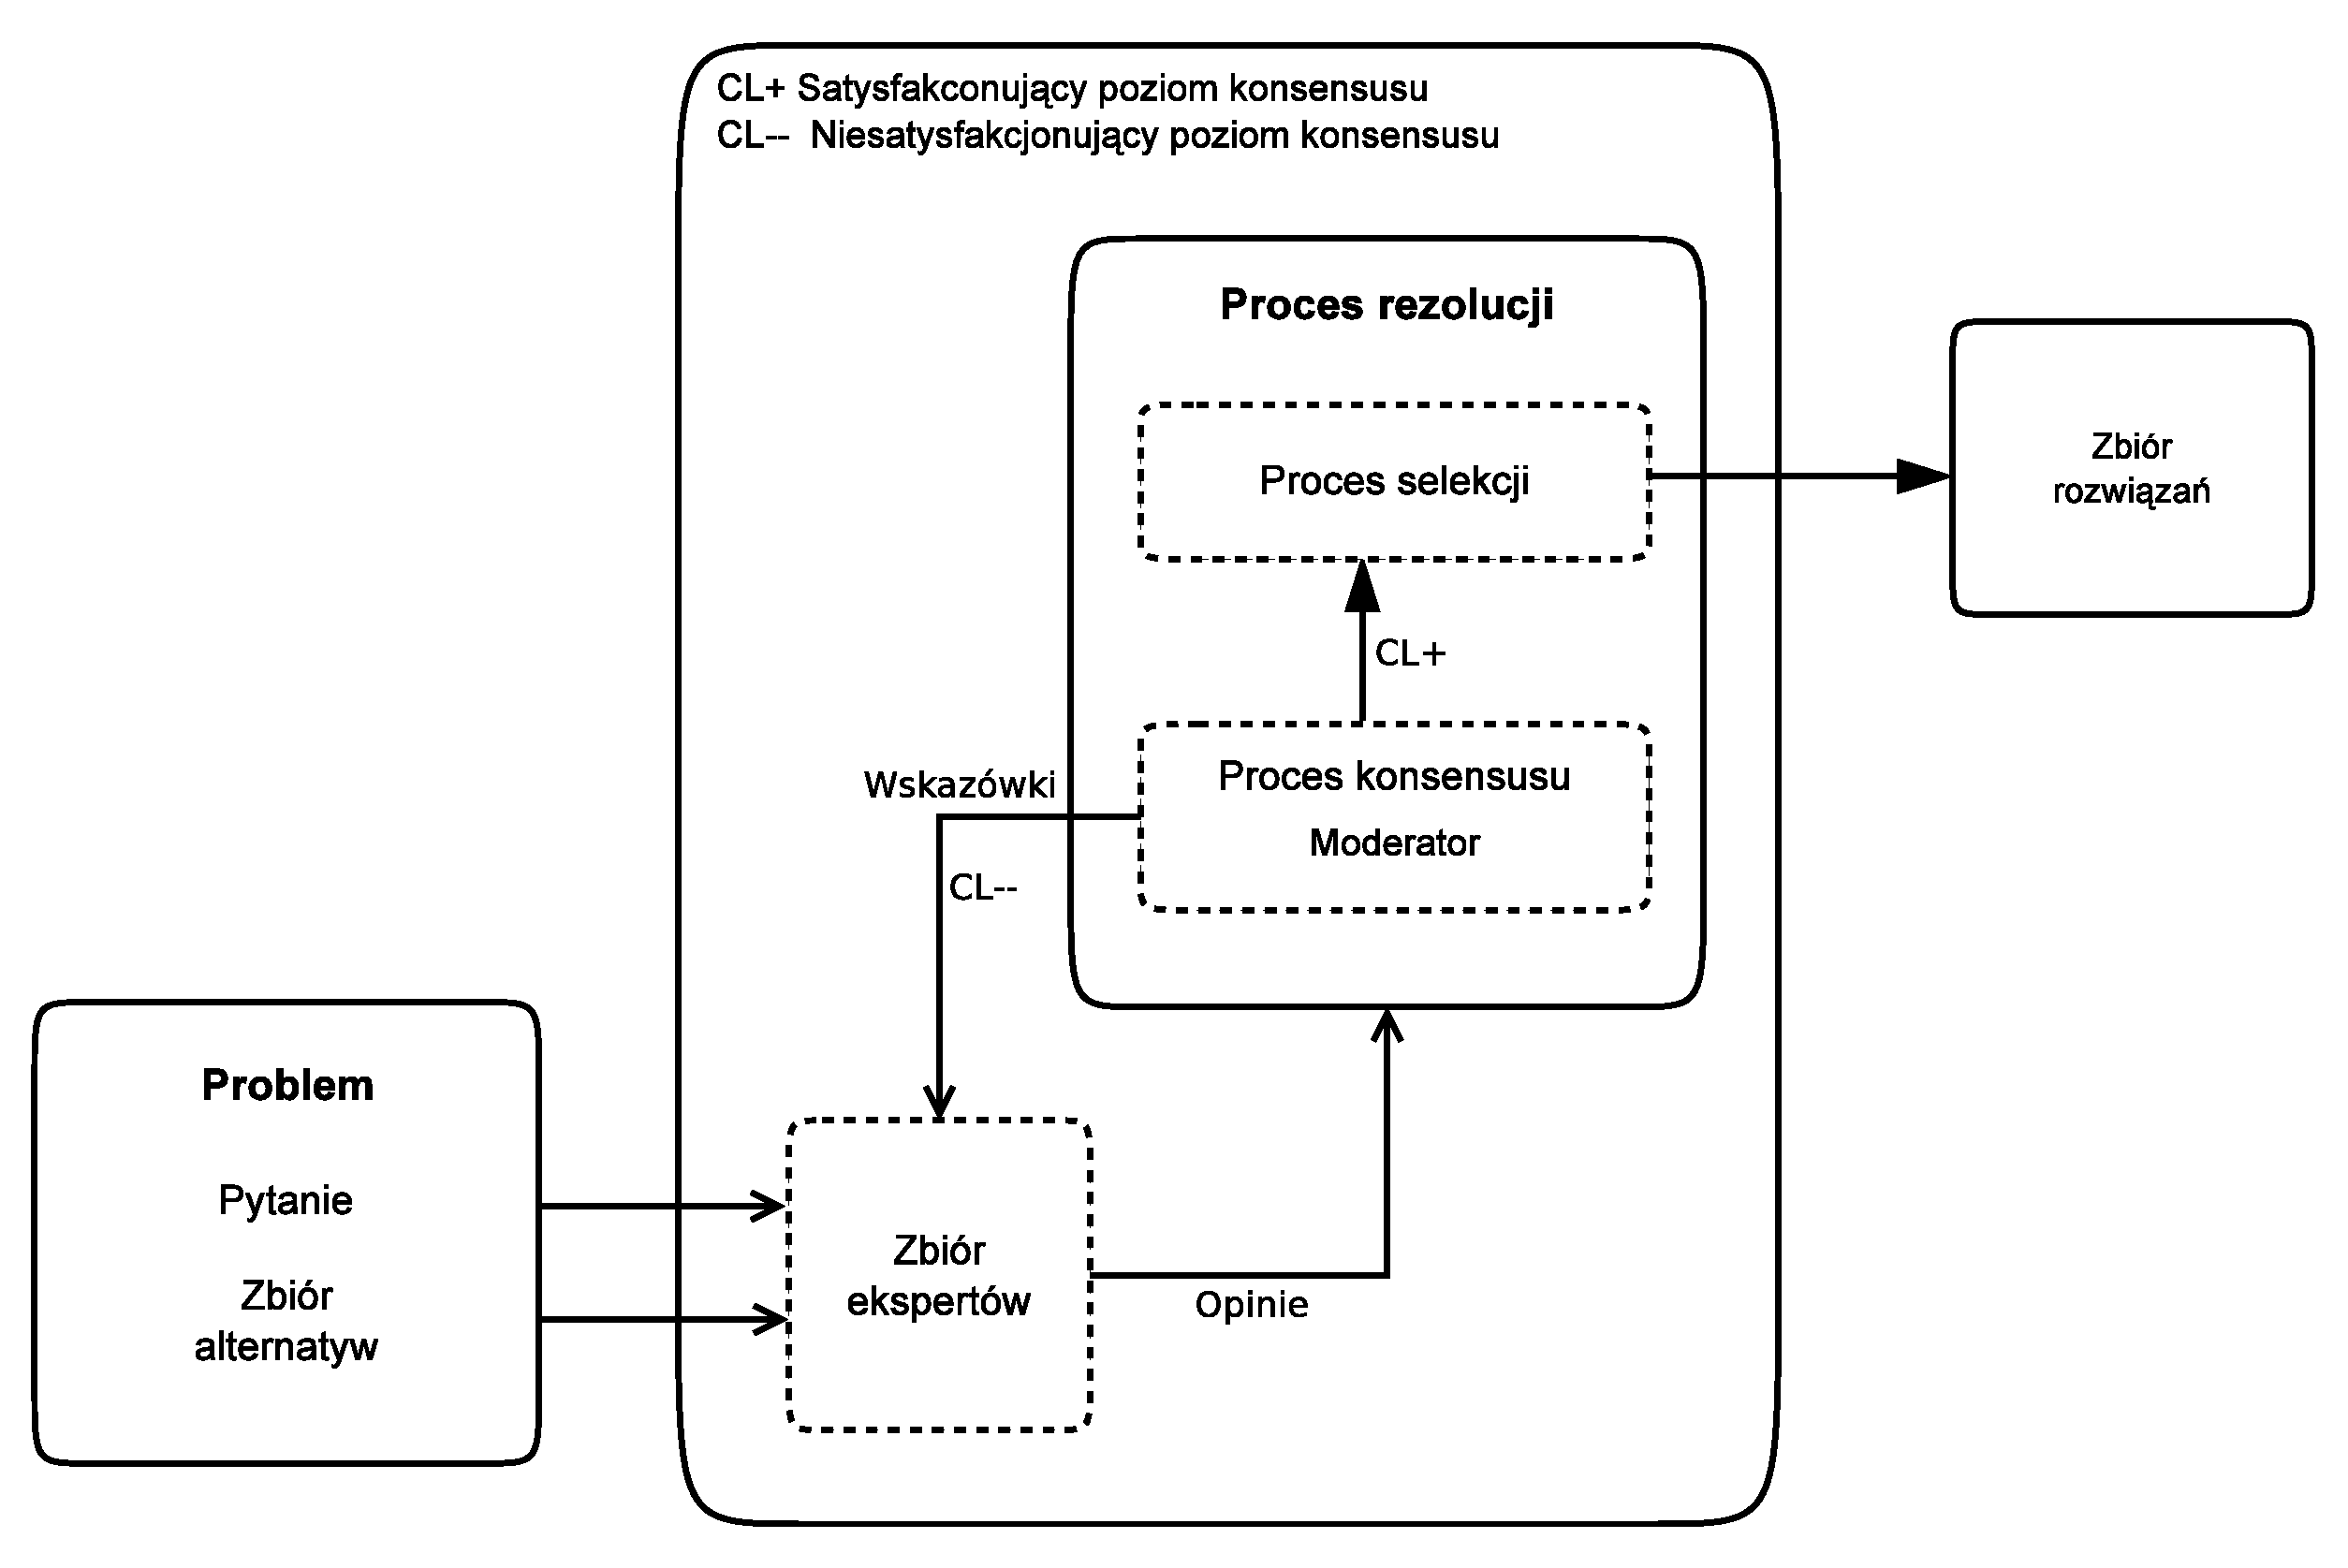
\includegraphics[width=\linewidth]
    {chapters/modelinggroupdecision/schemat_procesu-eps-converted-to.pdf}
  \caption{Procesy w grupowym podejmowaniu decyzji}
  \label{fig:Procesy_w_grupowym_podejmowaniu_decyzji}
\end{figure}

Typowy proces
porozumienia widoczny jest na rysunku
\ref{fig:Procesy_w_grupowym_podejmowaniu_decyzji}. Jest on zdefiniowany jako
dynamiczny proces iteracyjny i obejmuje następujący skończony zbiór kroków:
\begin{enumerate}[1.]
  \item Problem oraz zbiór możliwych alternatyw przedstawiane są ekspertom.
  
  \item \label{itm:2nd} Eksperci przedstawiają moderatorowi swoje preferencje
  przy użyciu określonego sposobu reprezentacji preferencji.
  
  \item Kiedy wszyscy przedstawią swoje preferencje, moderator sprawdza czy 
  poziom konsensusu wśród wszystkich ekspertów jest wystarczająco wysoki.
  
  \item 
  \begin{enumerate}[i)]
    \item Jeśli poziom konsensusu jest wystarczająco wysoki to proces się kończy
    i przechodzi do procesu selekcji (krok \ref{itm:6th}).
	\item Jeśli poziom konsensusu nie jest wystarczająco wysoki to moderator 
	udziela ekspertom wskazówek tak, aby mogli zmienić swoje preferencje i 
	osiągnąć konsensus.
  \end{enumerate}
  
  \item Biorąc pod uwagę zalecenia moderatora, eksperci zmieniają swoje
  preferencje co do alternatyw i rozpoczyna się nowa runda procesu (krok
  \ref{itm:2nd}).
  
  \item \label{itm:6th} Przejście do procesu selekcji i obliczenie
  ostatecznego rozwiązania.

\end{enumerate}

Warto zwrócić uwagę, że tak zdefiniowany proces konsensusu może przypominać 
klasyczną metodę delficką. Jednakże istnieje kilka istotnych różnic:
\begin{itemize}
  \item W metodzie delfickiej ostatecznym celem jest prognozowanie, podczas gdy 
  powyższe podejście próbuje znaleźć najlepszą alternatywę z zestawu możliwych.
  \item Zamiast kwestionariuszy, eksperci wyrażają swoje preferencje za pomocą 
  pewnych konkretnych formatów reprezentacji preferencji.
  \item Metoda delficka zakłada anonimowość uczestników, natomiast w 
  proponowanym modelu nie ma takiego ograniczenia.
\end{itemize}

W przedstawionym modelu bardzo ważna jest rola moderatora. W dalszej części 
pracy zostaną przedstawione narzędzia pozwalające zredukować jego pracę, a 
nawet go zastąpić. Kolejnym ważnym elementem jest sposób przedstawienia 
preferencji ekspertów. Temu tematowi poświęcony jest osobny rozdział.

\subsection{Proces selekcji}
Etap ten na wejściu dostaje oceny wszystkich ekspertów i jest odpowiedzialny za 
podanie kolejności rozwiązań. Proces selekcji można różnie definiować, w 
zależności od dokładnego umiejscowienia w modelu oraz zakresu odpowiedzialności 
procesu konsensusu. Zgodnie z Chiclana et al. [7] proces selekcji jest
podzielony na dwie fazy:
\begin{enumerate}
  \item Faza agregacji
  
  Faza ta definiuje globalne preferencje pomiędzy alternatywami wykorzystując 
  do tego techniki agregacji.
  
  \item Faza eksploatacji
  
  Faza ta przekształca zagregowaną globalną informację o preferencjach względem 
  alternatyw w globalny ranking. Sposób ustalenia rankingu jest dowolny i zależy
  od przyjętych technik reprezentacji preferencji i agregacji.

\end{enumerate}

\subsection{Moderator i mechanizm informacji zwrotnej}
Moderator jest osobą niebiorącą udziału w dyskusji w sposób bezpośredni. Jego
zadaniem jest kierowanie grupą, analizowanie wyników głosowań i na ich podstawie
wpływanie na na opinie ekspertów tak, aby został osiągnięty jak największy 
stopień konsensusu. Jak część modelu wprowadzony zostaje mechanizm informacji 
zwrotnej, który ma zastąpić osobę moderatora i zautomatyzować proces. Mechanizm 
składa się z kilku prostych zasad, które generują rekomendacje dla ekspertów. 
Aby to osiągnąć, wykorzystywane są miary przybliżone w połączeniu ze stopniem 
konsensusu. Na końcu, porady muszą zostać przedstawione w sposób czytelny dla 
człowieka, żeby eksperci mogli je wykorzystać do zmiany swoich poglądów.

\section{Dynamika: zbiór alternatyw}
Zazwyczaj metody rozwiązywania problemów grupowych są statyczne. Oznacza to 
założenie, że liczba alternatyw oraz ekspertów przez cały proces decyzyjny jest 
stała. Jednak w rzeczywistych sytuacjach okazuje się, że proces może być 
dynamiczny.

Szczególnie częstym zjawiskiem jest dynamika zbioru alternatyw. Typowym 
przykładem takiej sytuacji jest diagnoza lekarska. Środowisko to jest dynamiczne
w tym sensie, że pacjent może przedstawić nowe objawy lub mógł poczuć się lepiej
ze względu na przyjmowane leki, a więc każda zmiana stanu pacjenta powinna być 
brana pod uwagę przez lekarzy.

Aby proces decyzyjny stał się bardziej realistyczny, należy zdefiniować metodę, 
która pozwala usunąć i wstawić nowe alternatywy do procesu dyskusji. Ze względu 
na chęć wyeliminowania osoby moderatora, metoda ta powinna być maksymalnie 
zautomatyzowana.

\begin{figure}[ht]
  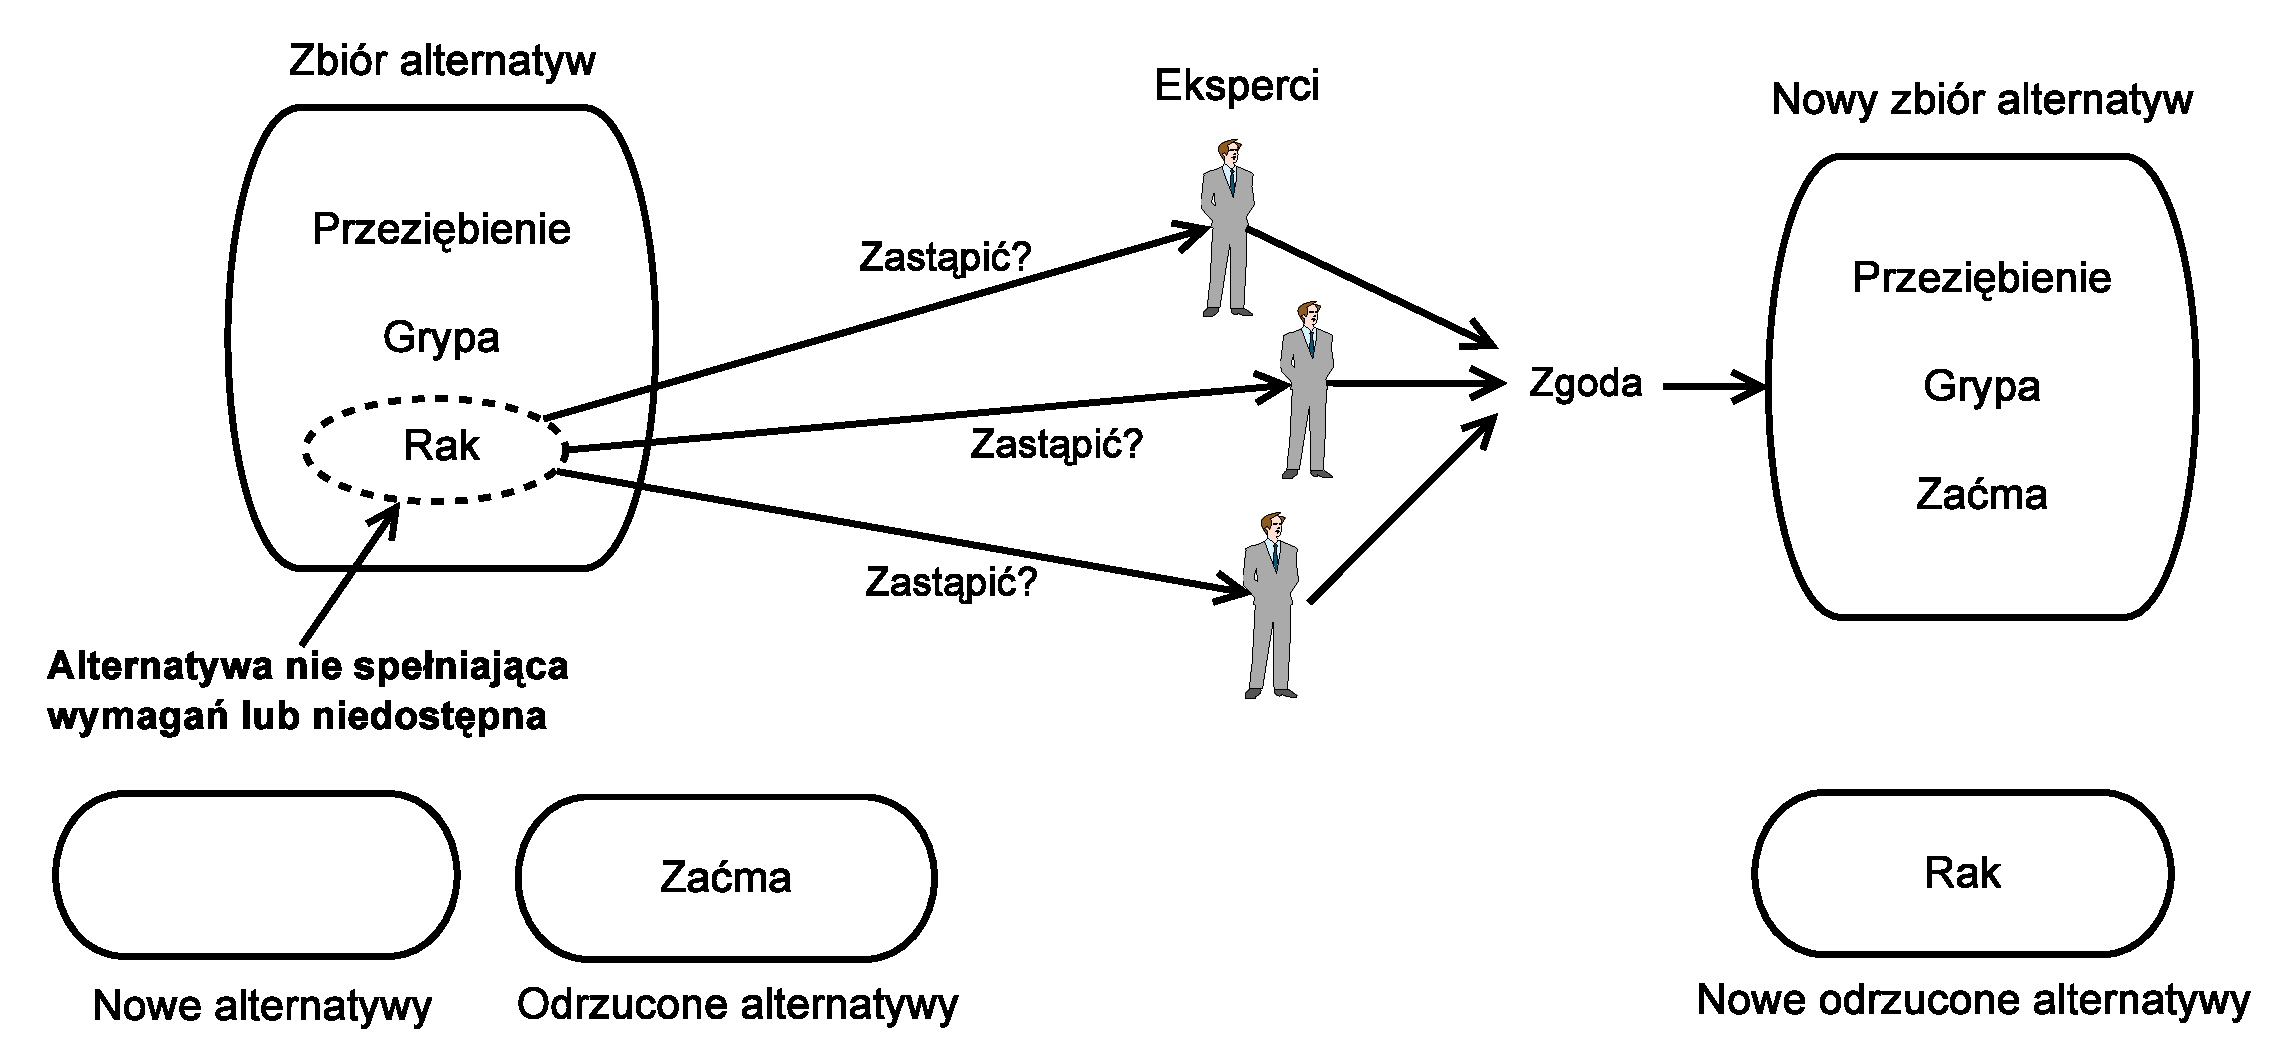
\includegraphics[width=\linewidth]
  	{chapters/modelinggroupdecision/usuniecie_alternatyw-eps-converted-to.pdf}
  \caption{Dynamika alternatyw: Usunięcie}
  \label{fig:dynamika_alternatyw_usuniecie}
\end{figure}

Wpierw, system identyfikuje rozwiązania najgorsze ze względu na oceny ekspertów,
które mogą zostać usunięte. Następnie szuka nowych, które może dołączyć. Nowe 
alternatywy można uzyskać z propozycji, które pojawiły się w trakcie dyskusji 
albo ze zbioru rozwiązań, które były dostępne od samego początku, ale nie 
zostały ujęte w dyskusji ze względu na nie spełnienie początkowych kryteriów 
problemu. Istnieje też możliwość ponownego włączenia do dyskusji alternatyw 
wcześniej usuniętych. Wyraźnie widać, że metoda dzieli się na dwie fazy: 
usunięcie nieaktualnych i złych alternatyw (rysunek
\ref{fig:dynamika_alternatyw_usuniecie}) oraz dodanie nowych alternatyw (rysunek
\ref{fig:dynamika_alternatyw_dodanie}).
W tak zdefiniowanej metodzie moderator jest zastąpiony przez system oraz samych decydentów, którzy muszą być informowani o 
zmianach i je akceptować.

\begin{figure}[ht]
  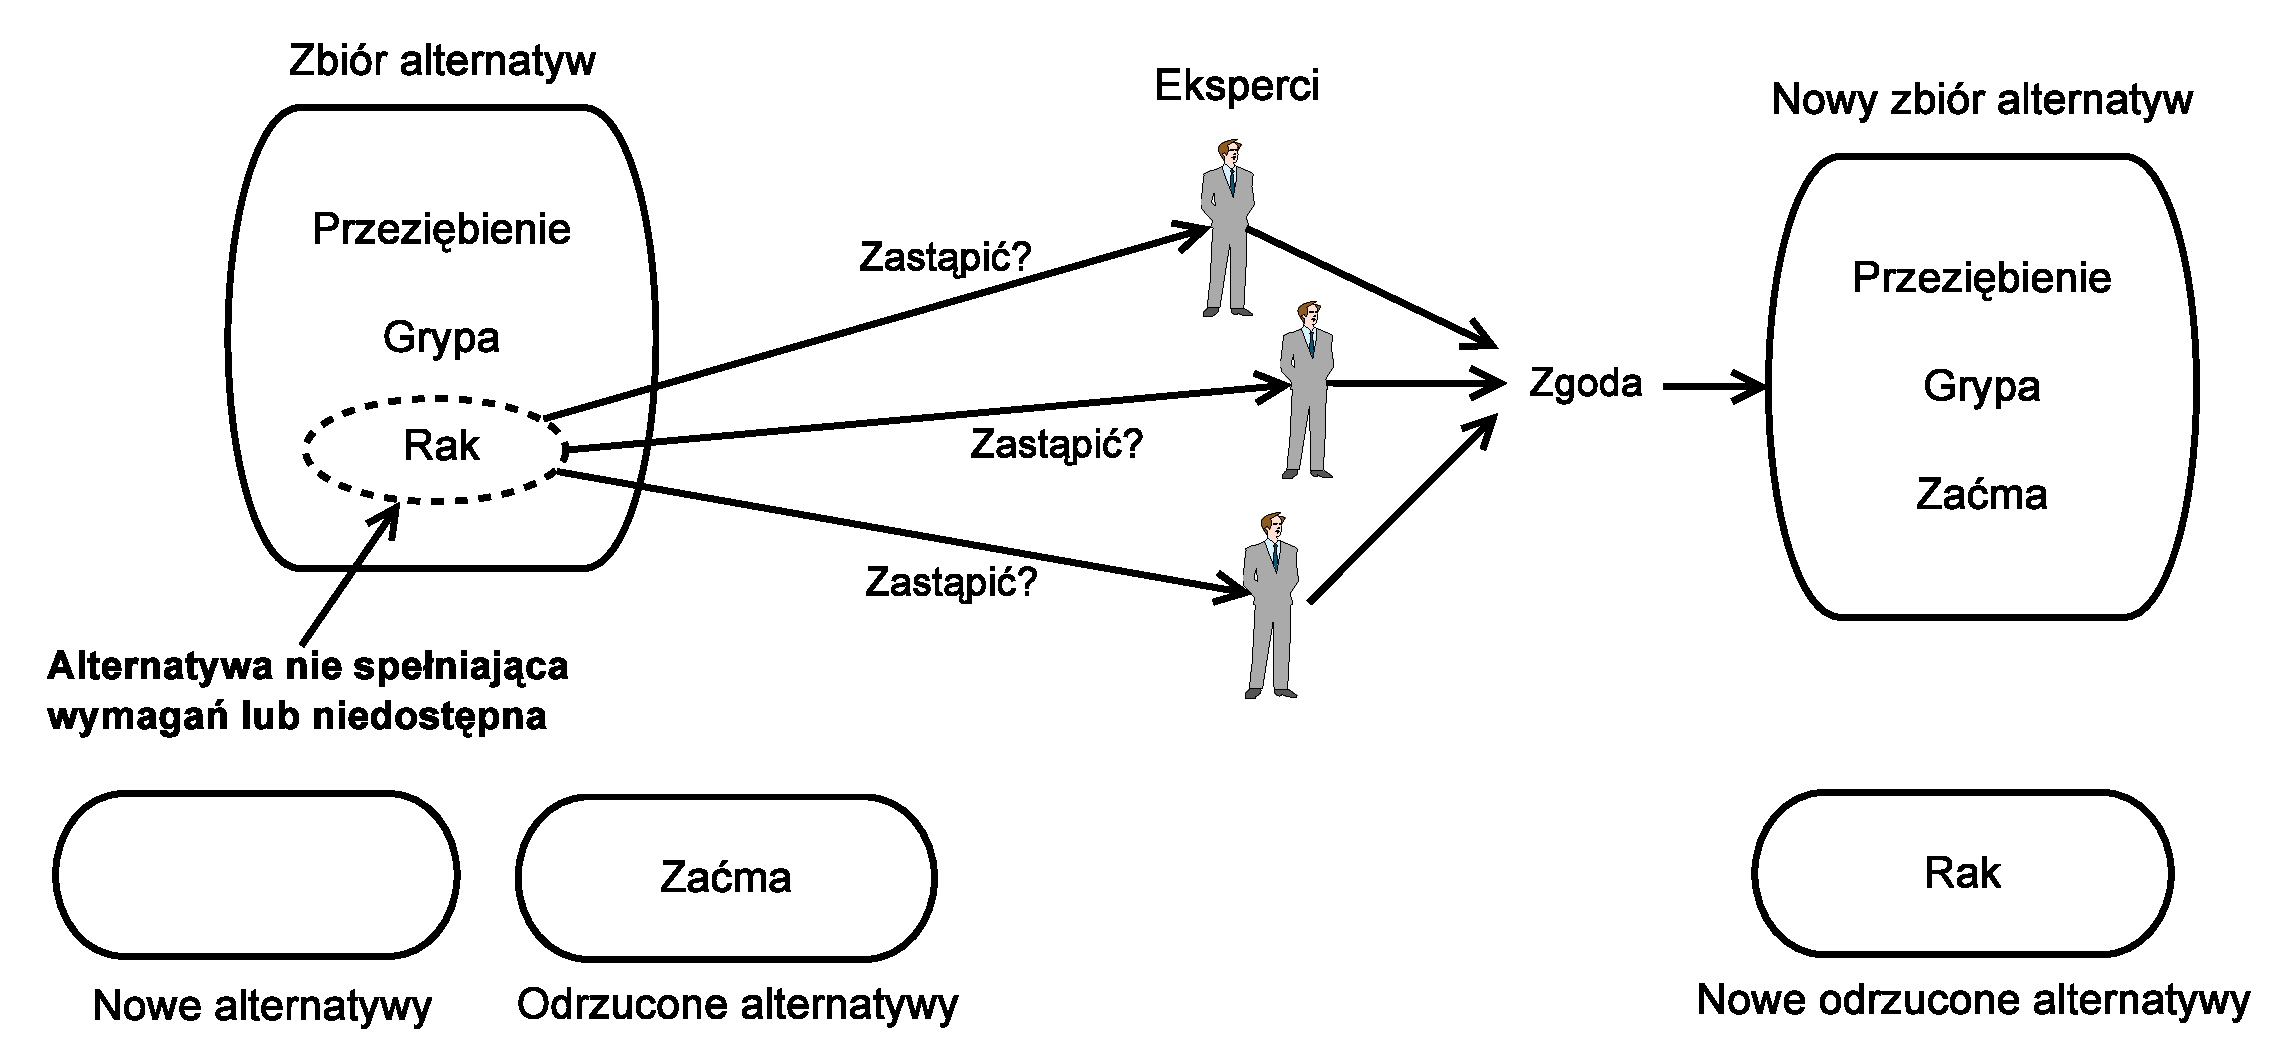
\includegraphics[width=\linewidth]
  	{chapters/modelinggroupdecision/usuniecie_alternatyw-eps-converted-to.pdf}
  \caption{Dynamika alternatyw: Dodanie}
  \label{fig:dynamika_alternatyw_dodanie}
\end{figure}

\section{Dynamika: zbiór ekspertów}
Kolejnym aspektem jest dynamiczny zbiór ekspertów. Przykładem może być grupa
lekarzy, którzy na pewnym etapie badań nie są w stanie postawić diagnozy i
proszą o konsultację z innym lekarzem lub lekarzami, którzy mogą mieć większe
doświadczenie w danej dziedzinie. Innym przykładem jest sytuacja, w której
członek grupy decydentów w firmie przebywał na urlopie i wraca do pracy w
trakcie trwania procesu decyzyjnego. Może się również zdarzyć, że jeden z
członków odchodzi z zespołu lub na jakiś czas wyłącza się z dyskusji. Oba
przypadki, dodanie oraz usunięcie decydenta, powinny być wspierane przez system
podejmowania decyzji i należy je rozpatrywać osobno. 

W przypadku pojawienia się nowego eksperta należy zastanowić się nad kilkoma
rzeczami. Po pierwsze, taka osoba powinna zostać zaakceptowana przez grupę.
Jedną z możliwości jest wysłanie zaproszenia przez jednego z członków. Takie
zaproszenie powinno wcześniej zostać zatwierdzone przynajmniej przez większość
grupy. Druga możliwość to chęć dołączenia do procesu ze strony nowej osoby bez
wiedzy grupy. W tym przypadku, system musi informować grupę o zaistniałej
sytuacji i czekać na informację zwrotną w sposób analogiczny do akceptacji
zaproszenia. Następny krok to zapoznanie z problemem i aktualnym stanem procesu
decyzyjnego. Ponownie istnieją dwie opcje: ujawnienie danych historycznych lub
nie. Jeżeli historia procesu jest niejawna (grupa może oczekiwać od nowej osoby
świeżego spojrzenia) to system przedstawia tylko aktualny zestaw alternatyw.
Jeżeli jednak z jakiś powodów przebieg dyskusji musi być jawny (na przykład
historia pacjenta i analiza możliwych przyczyn choroby) to system musi
przedstawić historię głosowań oraz zestawienie dodanych i odrzuconych
alternatyw. W tym celu można wykorzystać mechanizm informacji zwrotnej.

Kiedy ekspert odchodzi z grupy sytuacja jest dużo prostsza: system w kolejnej 
turze nie czeka na dane od takiej osoby. Ciekawszy przypadek to tymczasowe 
wycofanie się z procesu decyzyjnego. Członek grupy może zgłosić, że przez 
nieokreślony czas nie będzie głosował ani brał udziału w dyskusji. Mimo tego 
system powinien w dalszym ciągu informować o aktualnym stanie procesu. W tej 
pracy omawiane są szczególnie mobilne podejmowanie decyzji. Pociąga to za sobą 
spadek dynamiki procesu, ponieważ nie każdy z członków może brać czynny udział 
w dyskusji w tym samym momencie. Pomysłem jest umówienie się, że na głosowanie 
każdy z członków ma na przykład 24 godziny. Jeśli do tego czasu większość 
ekspertów udzieli odpowiedzi, to pozostali zostaną potraktowani tak, jakby 
tymczasowo się wycofali. Grupa sama musi zdecydować co oznacza większość (np. 
brak jednej osoby, dwóch albo zero) oraz ile czasu jest na odpowiedzi. Takie 
podejście zapobiega sztucznemu spowalnianiu procesu.


